\documentclass[]{article}
\usepackage{lmodern}
\usepackage{amssymb,amsmath}
\usepackage{ifxetex,ifluatex}
\usepackage{fixltx2e} % provides \textsubscript
\ifnum 0\ifxetex 1\fi\ifluatex 1\fi=0 % if pdftex
  \usepackage[T1]{fontenc}
  \usepackage[utf8]{inputenc}
\else % if luatex or xelatex
  \ifxetex
    \usepackage{mathspec}
  \else
    \usepackage{fontspec}
  \fi
  \defaultfontfeatures{Ligatures=TeX,Scale=MatchLowercase}
\fi
% use upquote if available, for straight quotes in verbatim environments
\IfFileExists{upquote.sty}{\usepackage{upquote}}{}
% use microtype if available
\IfFileExists{microtype.sty}{%
\usepackage{microtype}
\UseMicrotypeSet[protrusion]{basicmath} % disable protrusion for tt fonts
}{}
\usepackage[margin=1in]{geometry}
\usepackage{hyperref}
\PassOptionsToPackage{usenames,dvipsnames}{color} % color is loaded by hyperref
\hypersetup{unicode=true,
            pdftitle={W241 Final Report},
            pdfauthor={David Hou, Ravi Ayyappan, Ahsen Qamar},
            colorlinks=true,
            linkcolor=blue,
            citecolor=Blue,
            urlcolor=blue,
            breaklinks=true}
\urlstyle{same}  % don't use monospace font for urls
\usepackage{graphicx,grffile}
\makeatletter
\def\maxwidth{\ifdim\Gin@nat@width>\linewidth\linewidth\else\Gin@nat@width\fi}
\def\maxheight{\ifdim\Gin@nat@height>\textheight\textheight\else\Gin@nat@height\fi}
\makeatother
% Scale images if necessary, so that they will not overflow the page
% margins by default, and it is still possible to overwrite the defaults
% using explicit options in \includegraphics[width, height, ...]{}
\setkeys{Gin}{width=\maxwidth,height=\maxheight,keepaspectratio}
\IfFileExists{parskip.sty}{%
\usepackage{parskip}
}{% else
\setlength{\parindent}{0pt}
\setlength{\parskip}{6pt plus 2pt minus 1pt}
}
\setlength{\emergencystretch}{3em}  % prevent overfull lines
\providecommand{\tightlist}{%
  \setlength{\itemsep}{0pt}\setlength{\parskip}{0pt}}
\setcounter{secnumdepth}{0}
% Redefines (sub)paragraphs to behave more like sections
\ifx\paragraph\undefined\else
\let\oldparagraph\paragraph
\renewcommand{\paragraph}[1]{\oldparagraph{#1}\mbox{}}
\fi
\ifx\subparagraph\undefined\else
\let\oldsubparagraph\subparagraph
\renewcommand{\subparagraph}[1]{\oldsubparagraph{#1}\mbox{}}
\fi

%%% Use protect on footnotes to avoid problems with footnotes in titles
\let\rmarkdownfootnote\footnote%
\def\footnote{\protect\rmarkdownfootnote}

%%% Change title format to be more compact
\usepackage{titling}

% Create subtitle command for use in maketitle
\newcommand{\subtitle}[1]{
  \posttitle{
    \begin{center}\large#1\end{center}
    }
}

\setlength{\droptitle}{-2em}
  \title{W241 Final Report}
  \pretitle{\vspace{\droptitle}\centering\huge}
  \posttitle{\par}
  \author{David Hou, Ravi Ayyappan, Ahsen Qamar}
  \preauthor{\centering\large\emph}
  \postauthor{\par}
  \predate{\centering\large\emph}
  \postdate{\par}
  \date{April 2019}

\usepackage{float}

\begin{document}
\maketitle

\hypertarget{introduction}{%
\subsection{Introduction}\label{introduction}}

The importance of good sleep habits is emphasized quite often in
contemporary advice. One aspect of good sleep hygiene is the avoidance
of electronic devices with backlit screens prior to bed. The light from
these screens causes the brain to stay under the assumption of daytime,
inhibiting the production of the sleep hormone melatonin. In this
experiment, we seek a quantitative measure of sleep quality degradation
as a result of screen-time before bed. Due to our limited expertise and
resources for studying sleep science, we will perform the measaurement
using a mobile app.

\hypertarget{experiment-design}{%
\subsection{Experiment Design}\label{experiment-design}}

The app used is called \href{www.sleepcycle.com}{Sleep Cycle} and
utilizes the phone's microphone to measure a user's sleep cycles
overnight. It is primarily advertised for its alarm clock feature, which
attempts to wake a user in the lightest phase of sleep in a preset time
interval. Each morning, the app displays a graph of the user's sleep
cycles in the previous night and some relevant statistics. Figure
\ref{fig:example_night} shows an example of the output from one night's
data.

\begin{figure}[H]

{\centering 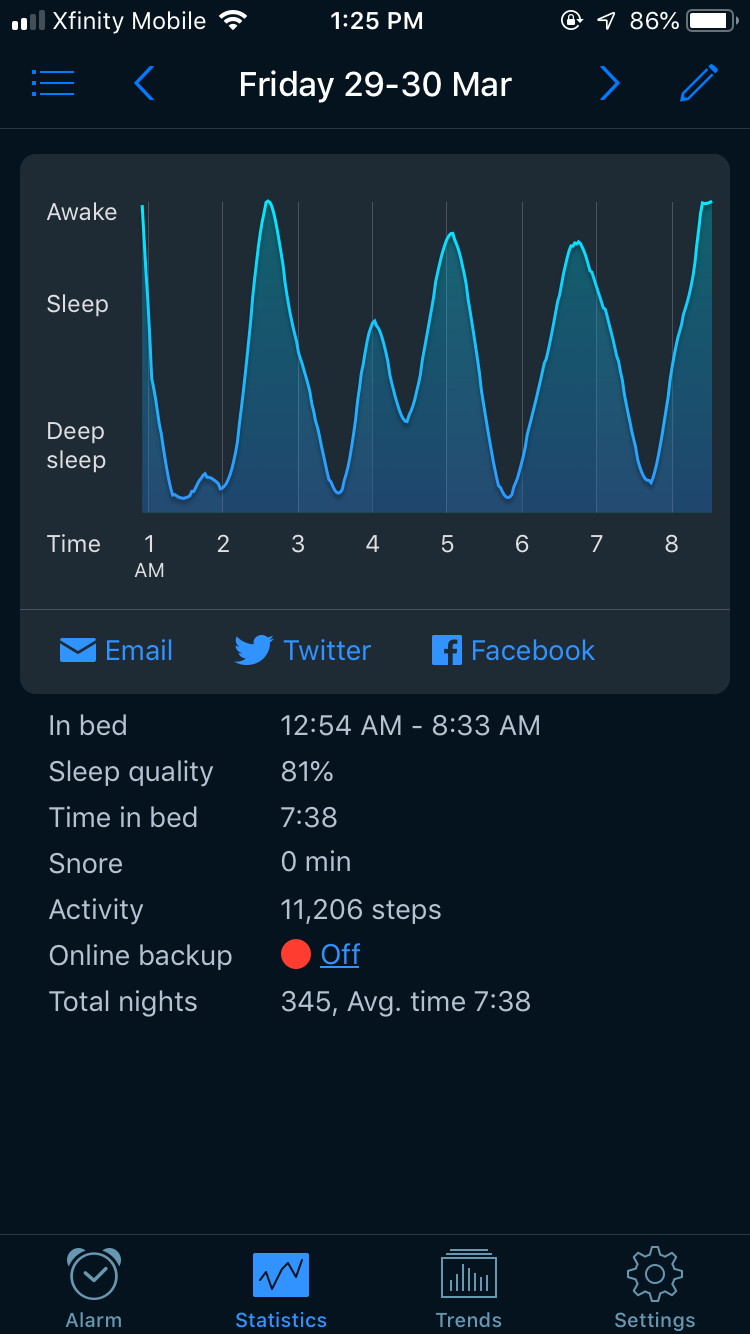
\includegraphics[width=0.25\linewidth]{img/example_night} 

}

\caption{Example night}\label{fig:example_night}
\end{figure}

One of these statistics is a ``Sleep Quality'' number, which is the
principle outcome variable in this experiment. According to the
\emph{Sleep Cycle} website, these four factors go into calculating Sleep
Quality:

\begin{enumerate}
\def\labelenumi{\arabic{enumi}.}
\tightlist
\item
  Amount of time spent in bed.
\item
  Amount of time spent in deep sleep.
\item
  Consistency of the sleep.
\item
  Amount of times where the app registered you as fully awake.
\end{enumerate}

Of the four factors, users generally only have direct control over the
first one. In order to be less intrusive, we did not control the amount
of time that users spend in bed, but we did instruct subjects to try to
sleep at regular hours every night. The other three factors are
hopefully affected by screen-time, allowing us to measure a treatment
effect. The app also records a ``snore'' and ``steps walked'' value, but
we have doubts about the accuracy of these measures and will not use
them in our analysis.

The experiment took place over two weeks, from March 23 to April 5 of
2019. Saturday was chosen as the start day of the week because it was
feared that instructions to change sleep habits in the middle of the
week might be ignored. We recruited 35 people for the study using a
Google survey, consisting of classmates, friends, and family. In
addition to asking for contact and demogrphic information, the survey
also inquired about general sleep habits such as bedtime and pre-sleep
activities. While the survey did ask about electronic usage, the
questions were mixed in among other questions such as workout habits and
alcohol consumption. Prior to commencement of the experiment, subjects
were not made aware of the fact that screen-time was the critical
variable of interest.

All communications to subjects occurred over email. Every person in the
same experimental group received identical emails (see Appendix). When
instructing subjects to use electronics prior to bed, we did not mandate
any specific activity, as we felt it would increase non-complicance on
an already-intrusive study. We only specified that users should use some
sort of eletronic device with a backlit screen for 30 minutes
immediately before bedtime. Similarly, we did not ask subjects in the
other group to perform anything in lieu of elctronic usage. These
subjects were simply asked to refrain from using electronics with
backlit screens 30 minutes before bedtime.

Subjects were assigned randomly to two groups, with group 1 receiving
treatment (screen-time before bed) during the first week and group 2
receiving control (no screen-time before bed). After the first week,
subjects were instructed to swap to the opposite activity of what they
were assigned to initially. The swapping design allows us to perform
within-subject comparisons while also leaving time for treatment effects
to manifest themselves. With the group that received treatment first, we
are also able to perform some analysis on persistence effects. Note that
subjects were not informed of the instruction swap ahead of time, so we
do not expect any anticipation effects.

The nature of experiment requires effort from subjects in both treatment
and control. That is, for people who normally use electronic devices
before bed, the request to refrain from useage constitutes a significant
change in pre-sleep ritual; for people who normally avoid electronics
before bed, the opposite is true. Therefore, we are concerned with
two-sided non-compliance, which is especially difficult to measure in
this experiment because people are unlikely to honestly report when they
have deviated from our instructions. To help combat this somewhat, we
offered subjects some small monetary compensation and emphasized
prioritization of honesty of compliance in reporting data. Even so, we
can never be sure of whether subjects followed instructions.

\hypertarget{experiment-deviations}{%
\subsubsection{Experiment Deviations}\label{experiment-deviations}}

Between the closing the sign-up survey, we asked all respondents to
begin using the app in order to establish baseline data and help the app
calibrate (the website claims that the app becomes more accurate over
time). Sleep habits during this baseline usage were not closely
controlled or monitored, as each subject signed up for the experiment at
different dates. However, we did ask for an export of this baseline data
prior to starting the experiment, so that subjects had some awareness of
the steps it takes to perform the export. At this time, we learned that
Android users could not perform the export due to missing functionality
in the app. As such, we asked Android users (4 out of the 38) to
manually record the sleep times and quality from the app each day.

After closing the sign-up survey, we decided to also included ourselves
as subjects in the experiment. This was to slightly raise the number of
subjects and out of curiosity for the effects on ourselves. Though we
were not aware of our own randomization a priori, we obviously had more
knowledge of the experiment than other subjects, so we will analyze our
own data with special care.

\hypertarget{results}{%
\subsection{Results}\label{results}}

\hypertarget{data-cleaning}{%
\subsubsection{Data Cleaning}\label{data-cleaning}}

We made as little modification to the raw data as possible, but a few
exceptions exist. We decided to omit entries for which the subject slept
for a duration shorter than one hour. On case by case basis, we
determined that these entries were caused by improper usage of the app.
There were several entries where the user had two entries in one night,
separated by some period of awakeness. In these cases, one or both of
the periods of sleep were also very short. However, none of them fell
under the one hour threshold for omission.

Of the 38 people who originally signed up for the study, only 29 people
actually submitted final data by the time of writing this report. As
such, we excluded their results. Note that these subjects are not
necessarily attriters, as we could not collect data from treatment or
control.

\hypertarget{analysis}{%
\subsubsection{Analysis}\label{analysis}}

Figure \ref{fig:quality_by_treatment_fig} shows the sleep quality,
averaged over the respective time periods, for each treatment
assignment. As mentioned above, the baseline data was collected in the
time between subjects signing up and the experiment officially starting.
We did not tightly control baseline data and not every subject provided
it.

\begin{figure}
\centering
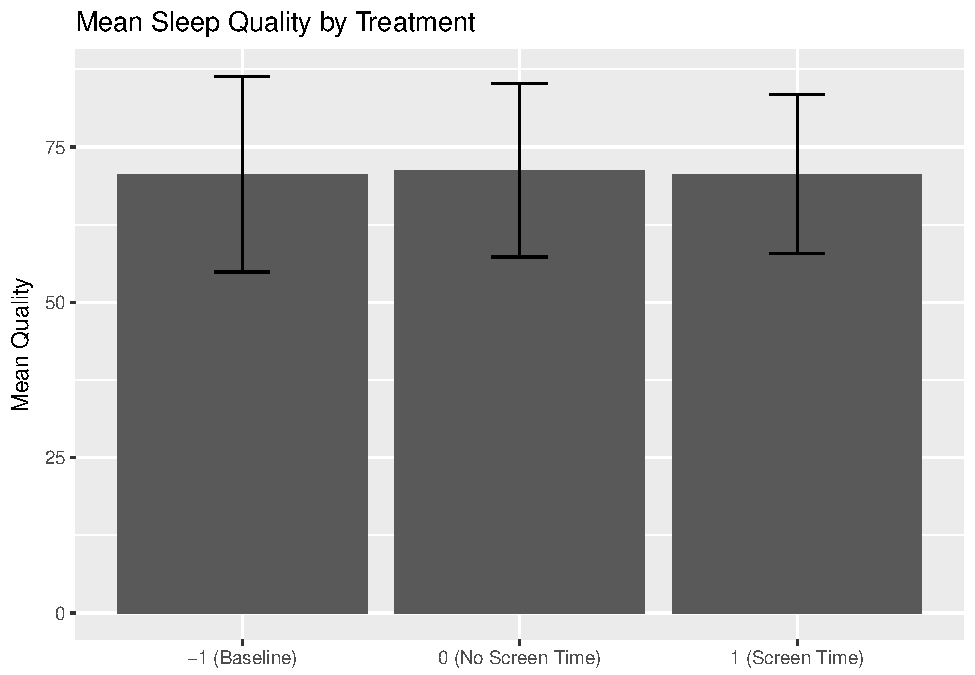
\includegraphics{report_files/figure-latex/quality_by_treatment_fig-1.pdf}
\caption{\label{fig:quality_by_treatment_fig} Mean sleep quality by
treatment}
\end{figure}

It is already clear that our experiment is too underpowered to detect a
treatment effect, as the error bars are extremely large comapred to the
barely noticeable differences in means. Table
\ref{tab:quality_by_treatment_tab} shows the tabular results for Figure
\ref{fig:quality_by_treatment_fig}. The point estimate for screen time
is slightly lower than that of no screen time, but the standard error is
way too large for this difference to be statistically significant.

\begin{table}[!htbp] \centering 
  \caption{\label{tab:quality_by_treatment_tab} Mean sleep quality by treatment} 
  \label{} 
\begin{tabular}{@{\extracolsep{5pt}} ccc} 
\\[-1.8ex]\hline 
\hline \\[-1.8ex] 
Label & Mean & St. Dev. \\ 
\hline \\[-1.8ex] 
Baseline & $70.608$ & $15.714$ \\ 
No Screen Time & $71.246$ & $13.944$ \\ 
Screen Time & $70.618$ & $12.806$ \\ 
\hline \\[-1.8ex] 
\end{tabular} 
\end{table}

Figure \ref{fig:quality_by_date_group1_fig} and Figure
\ref{fig:quality_by_date_group2_fig} show the mean sleep quality by
dates for the two groups. Recall that group 1 received treatment (screen
time) in week 1 of the experiment and switched to control (no screen
time) in week 2. Group 2 had the opposite schedule. Again, the large
error bars make it hard to draw any sort of conclusion for whether the
switch in treatment has any effect.

\begin{figure}
\centering
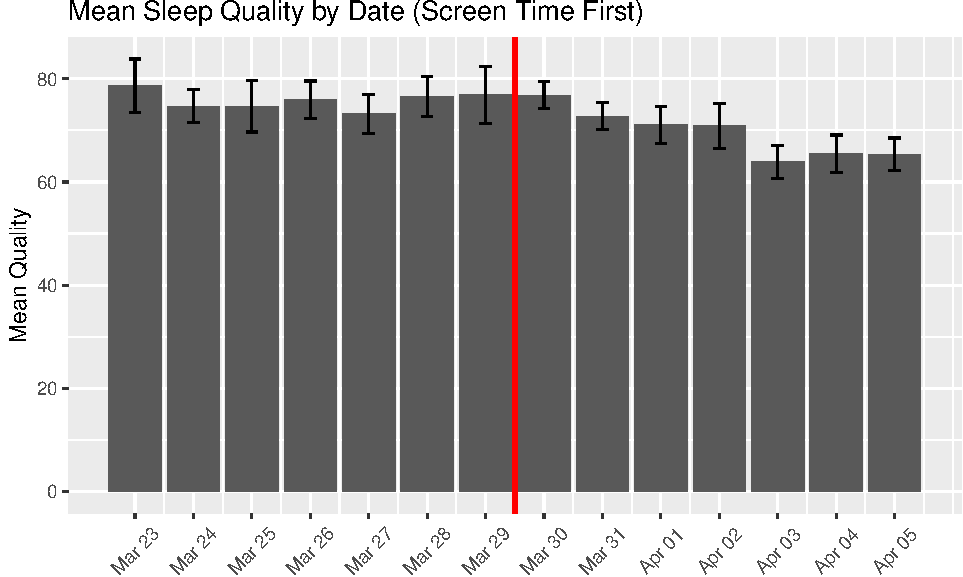
\includegraphics{report_files/figure-latex/quality_by_date_group1_fig-1.pdf}
\caption{\label{fig:quality_by_date_group1_fig} Mean sleep quality by
date in group which received screen time first}
\end{figure}

\begin{figure}
\centering
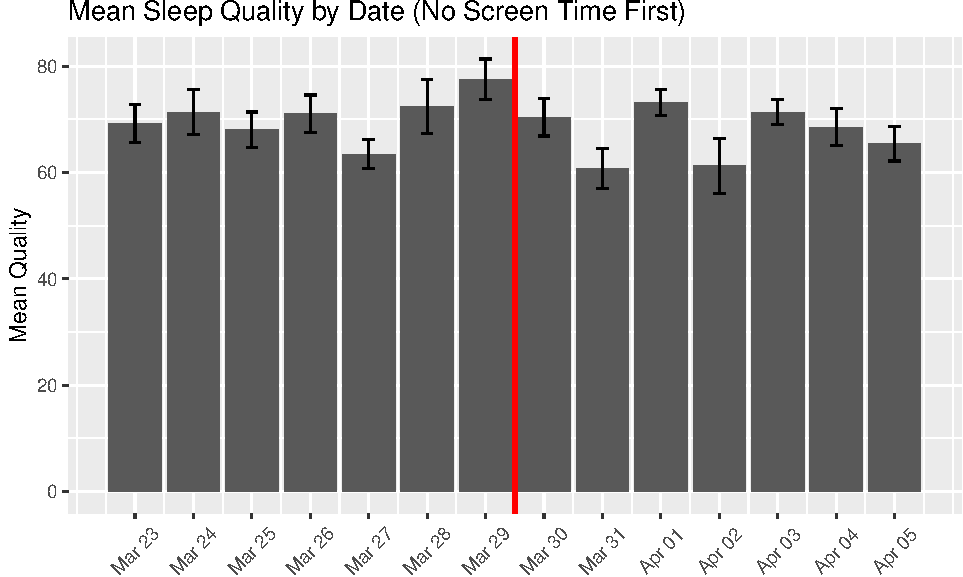
\includegraphics{report_files/figure-latex/quality_by_date_group2_fig-1.pdf}
\caption{\label{fig:quality_by_date_group2_fig} Mean sleep quality by
date in group that received no screen time first}
\end{figure}

Table \ref{tab:regressions} shows the results of three regressions
models:

\begin{enumerate}
\def\labelenumi{\arabic{enumi}.}
\tightlist
\item
  \(quality = \beta_0 + \beta_1 treat\)
\item
  \(quality = \beta_0 + \beta_1 treat + \beta_2 hours\)
\item
  \(quality = \beta_0 + \beta_1 treat + \beta_2 hours + \beta_3 id\)
\end{enumerate}

The covariates refer to treatment, hours slept, and unique indicators
for each person in the study. As expected, none of them show
statistically significance of the treatment (screen-time before bed)
affecting sleep quality. The number of hours slept and the specific
person has way more effect on sleep quality.

\begin{table}[!htbp] \centering 
  \caption{\label{tab:regressions} Regressions} 
  \label{} 
\begin{tabular}{@{\extracolsep{5pt}}lccc} 
\\[-1.8ex]\hline 
\hline \\[-1.8ex] 
 & \multicolumn{3}{c}{\textit{Dependent variable:}} \\ 
\cline{2-4} 
\\[-1.8ex] & \multicolumn{3}{c}{quality} \\ 
\\[-1.8ex] & (1) & (2) & (3)\\ 
\hline \\[-1.8ex] 
 Treatment (Screen-time) & 0.628 & $-$0.358 & $-$0.545 \\ 
  & (1.468) & (0.986) & (0.983) \\ 
  & & & \\ 
 Hours Slept &  & 8.014$^{***}$ & 7.889$^{***}$ \\ 
  &  & (0.396) & (0.397) \\ 
  & & & \\ 
 Subject ID &  &  & 0.139$^{**}$ \\ 
  &  &  & (0.058) \\ 
  & & & \\ 
 Constant & 70.618$^{***}$ & 14.085$^{***}$ & 13.172$^{***}$ \\ 
  & (1.071) & (2.888) & (2.893) \\ 
  & & & \\ 
\hline \\[-1.8ex] 
Observations & 336 & 336 & 336 \\ 
R$^{2}$ & 0.001 & 0.551 & 0.559 \\ 
Adjusted R$^{2}$ & $-$0.002 & 0.549 & 0.555 \\ 
Residual Std. Error & 13.424 (df = 334) & 9.009 (df = 333) & 8.947 (df = 332) \\ 
F Statistic & 0.183 (df = 1; 334) & 204.530$^{***}$ (df = 2; 333) & 140.133$^{***}$ (df = 3; 332) \\ 
\hline 
\hline \\[-1.8ex] 
\textit{Note:}  & \multicolumn{3}{r}{$^{*}$p$<$0.1; $^{**}$p$<$0.05; $^{***}$p$<$0.01} \\ 
\end{tabular} 
\end{table}

\hypertarget{conclusion}{%
\subsection{Conclusion}\label{conclusion}}

This experiment was too small to demonstrate any statistically
significant treatment effect. It would be interesting to repeat this
test with a much larger population.


\end{document}
